% (u)pLaTeX 非互換なパッケージ使用時に自動でパッチが適用される
\RequirePackage{plautopatch}

% uplatex オプションを指定し、ユニコード対応に。ただし、uplatex でコンパイルすること。
% ここで dvipdfmx を指定すれば、graphicx などでは指定しなくて良い。
\documentclass[oneside,openright,a4paper,papersize,uplatex,dvipdfmx]{jsarticle}
% \documentclass[english]{jsbook}

% 修論本体と表紙で共通で必要となる設定
% jsbookで余白が広すぎるのを直す
% 参照 https://web.archive.org/web/20230119032705/https://oku.edu.mie-u.ac.jp/~okumura/jsclasses/
% https://github.com/texjporg/jsclasses
\setlength{\textwidth}{\fullwidth}
\setlength{\evensidemargin}{\oddsidemargin}
\addtolength{\textwidth}{-5truemm}
\addtolength{\oddsidemargin}{5truemm}

% 同梱の ISEE 用の表紙テンプレ
\usepackage{thesis_cover}

% 色
\usepackage[dvipdfmx]{color}

% OTF フォントを使えるようにし、複数のウェイトも使用可能にする。
% これがないと、Mac のヒラギノ環境で使われる角ゴが太すぎてみっともない。
\usepackage[deluxe]{otf}

% OT1→T1に変更し、ウムラウトなどを PDF 出力で合成文字ではなくす
\usepackage[T1]{fontenc}

% uplatex の場合に必要な処理 
\usepackage[utf8]{inputenc} % エンコーディングが UTF8 であることを明示する。
\usepackage[prefernoncjk]{pxcjkcat} % アクセントつきラテン文字を欧文扱いにする

% Helvetica と Times を sf と rm のそれぞれで使う。
% default だとバランスが悪いので、日本語に合わせて文字の大きさを調整する。
\usepackage[scaled=1.05,helvratio=0.95]{newtxtext}

% latexdiff
% 実際の修論には入れる必要なし
%DIF PREAMBLE EXTENSION ADDED BY LATEXDIFF
%DIF UNDERLINE PREAMBLE %DIF PREAMBLE
\RequirePackage[normalem]{ulem} %DIF PREAMBLE
\RequirePackage{color}\definecolor{RED}{rgb}{1,0,0}\definecolor{BLUE}{rgb}{0,0,1} %DIF PREAMBLE
\providecommand{\MyDIFadd}[1]{{\protect\color{blue}\uwave{#1}}} %DIF PREAMBLE
\providecommand{\MyDIFdel}[1]{{\protect\color{red}\sout{#1}}}                      %DIF PREAMBLE
%DIF SAFE PREAMBLE %DIF PREAMBLE
\providecommand{\MyDIFaddbegin}{} %DIF PREAMBLE
\providecommand{\MyDIFaddend}{} %DIF PREAMBLE
\providecommand{\MyDIFdelbegin}{} %DIF PREAMBLE
\providecommand{\MyDIFdelend}{} %DIF PREAMBLE
%DIF FLOATSAFE PREAMBLE %DIF PREAMBLE
\providecommand{\MyDIFaddFL}[1]{\MyDIFadd{#1}} %DIF PREAMBLE
\providecommand{\MyDIFdelFL}[1]{\MyDIFdel{#1}} %DIF PREAMBLE
\providecommand{\MyDIFaddbeginFL}{} %DIF PREAMBLE
\providecommand{\MyDIFaddendFL}{} %DIF PREAMBLE
\providecommand{\MyDIFdelbeginFL}{} %DIF PREAMBLE
\providecommand{\MyDIFdelendFL}{} %DIF PREAMBLE
%DIF END PREAMBLE EXTENSION ADDED BY LATEXDIFF


% 引用文献の形式を Okumura (2019) から [1] のように変更する場合はコメントを外す
\def\bynumber{1}

% 各節の番号を消す
\setcounter{secnumdepth}{0}

% citep や citet を有効にする
\ifdefined\bynumber
\usepackage[square,numbers]{natbib} % \bynumber が有効の場合は [1] のようにする
\else
\usepackage{natbib}
% (Okumura, 2009) などを (Okumura 2009) とする
% 日本語文章で全角丸括弧の表示にし、かつ \inhibitglue で役物同士の字間を適切にする。
% https://okumuralab.org/tex/mod/forum/discuss.php?d=2349
\setcitestyle{aysep={},notesep={},open={\inhibitglue(},close={)\inhibitglue}}
\fi

\makeatletter
\newcommand{\mysub}[2][]% #1=caption (optional), #2=graphics
{\bgroup
  \sbox0{#2}\usebox0
  \dimen0=\dimexpr \textwidth-\wd0\relax
  \ifx\\\@centercr \divide\dimen0 by 2\fi
  \sbox1{\begin{minipage}[t]{\dimen0}
    \subcaption{#1}%
  \end{minipage}}%
  \rlap{\raisebox{\dimexpr \ht0-\ht1}[0pt][0pt]{\usebox1}}\allowbreak
\egroup}
\makeatother

% 画像の取り扱いに必要
\usepackage{graphicx}

% 表でセルを複数列で結合する
\usepackage{multicol}

% 数式の機能を拡張
\usepackage{amsmath}

% 単位の記述を楽にする
\usepackage{siunitx}

% 化学式の記述を楽にする
\usepackage[version=4]{mhchem}

% bibliography を目次に追加
\usepackage[nottoc,notlot,notlof]{tocbibind}

% tableのパッケージ
\usepackage{tabularx}

% 文中に回り込んで図を配置する
\usepackage{wrapfig}

%% % SI単位系の単位を表示する
%% \usepackage{siunitx}

% subfigure 環境で、(a)、(b) などの番号を左上に表示する。宇宙系の分野ではこれが一般的なはず。
% \usepackage[nooneline]{subfigure}
% \subfiguretopcaptrue
\usepackage{subcaption} % subcaption は従来のsubfigure、subfigを置き換える新しいパッケージ

% Latex標準の罫線を微妙に改善する。(u)platexでは欧文用パッケージとの整合性をよくする
\usepackage{array}

% \text...をtc...にした命令が数式モードで使えるようにする
\usepackage{mathcomp}

% 行番号を表示する。添削時のみに使い、事務提出版ではコメントアウトする
%\usepackage{lineno}
%\linenumbers

% PDF 内で外部リンクや文書内リンクを生成したい場合に使う(好みによる)
% 印刷時に色が出るかどうかは、使用する PDF viewer の挙動による。
% 紙媒体で修論を提出する場合、文字色は黒にするのが適切なので要注意。
\usepackage[colorlinks=true,allcolors=blue]{hyperref}
% 色を個別に変更したい場合の例(あまり勧めない)
%\hypersetup{
%    colorlinks=true,
%    citecolor=red,
%    linkcolor=blue,
%    urlcolor=green,
%}

% こうするだけだと、文字に色をつけないが、リンク機能があると判断しにくい。
% hidelinks を消すと PDF 中のリンクを枠で囲む。
%\usepackage[hidelinks]{hyperref}

% PDF 内のしおりの文字化けを防ぐ
% 先頭に \RequirePackage{plautopatch} を追加すれば 2020 年以降の TeX 環境では不要
\usepackage{pxjahyper}

% newcommand を使うことで、繰り返し使う長ったらしい入力を簡単にすることができる
\makeatletter
\newcommand{\ion}[2]{#1$\;${\small\rmfamily\@Roman{#2}}\relax}%
\makeatother
\newcommand{\bs}{\symbol{92}} % backslash
\newcommand{\red}[1]{\textcolor{red}{#1}}
\newcommand{\ured}[1]{\textcolor{red}{\underline{\textcolor{black}{#1}}}}
\newcommand{\ugreen}[1]{\textcolor{green}{\underline{\textcolor{black}{#1}}}}
\newcommand{\ublue}[1]{\textcolor{blue}{\underline{\textcolor{black}{#1}}}}
\newcommand{\be}{\begin{equation}}
\newcommand{\ee}{\end{equation}}
\usepackage{acronym}
\newacro{PDE}{Photon Detection Efficiency}
\newacro{MS}{Mass Spectrometer}
\newacro{SiPM}{Silicon Photomultiplier}
\newacro{LXe}{Liquid Xenon}
\newacro{PSI}{Paul Scherrer Institute}
\newacro{CDCH}{Cylindrical Drift Chamber}
\newacro{pTC}{Pixelated Timing Counter}
\newacro{RDC}{Radiative Decay Counter}
\newacro{COBRA}{COnstant Bending RAdius}

% 氏名などの情報が入っているファイル。各自で編集。
\renewcommand{\thefootnote}{\fnsymbol{footnote}}
\title{2025年度 森・大谷研 メンバー紹介}
\date{2025年4月} % 日付(入れたくなければ空欄)
\seireki{2025} % 年度
\author{小川拓泰\footnote{e-mail: hogawa@icepp.s.u-tokyo.ac.jp} ,神山大樹\footnote{e-mail: kmymski@icepp.s.u-tokyo.ac.jp} ,高津大誠\footnote{e-mail: taisei@icepp.s.u-tokyo.ac.jp} ,馬越隆成\footnote{e-mail: umakoshi@icepp.s.u-tokyo.ac.jp}} % 氏名
\seifuku{} % 正本か副本か(このファイルでは変更する必要なし)

\renewcommand{\thefootnote}{\arabic{footnote}}

\begin{document}

\maketitle


% これを入れることでページ番号が表示されない。
%% \thispagestyle{empty}

\tableofcontents
%% \listoffigures
%% \listoftables

% input を使うことで、別ファイルに分割することができます。
\section{イントロダクション}

本資料は2025年に大谷・末原研究室(仮名)\footnote{
これまで森・大谷研究室と呼んでいたので筆者には少し違和感があるが、時期慣れるだろう。
}に入る学生が少しでも早く研究室に慣れるために用意した。大谷・末原研の研究室メンバーや研究内容に関して紹介する。


\section{プロジェクト紹介}

\subsection{ILC計画}
aaa
\subsection{US-Japanカロリメータ開発}
aaa
\subsection{MEG II実験}
aaa
\subsection{次世代$\mu^{+}\rightarrow e^{+}\gamma$探索実験}
aaa
\subsection{PIONEER実験}
aaa
\section{メンバー紹介}
aaa
\subsection{大谷航准教授}
aaa

\begin{figure}[h]
  \centering
  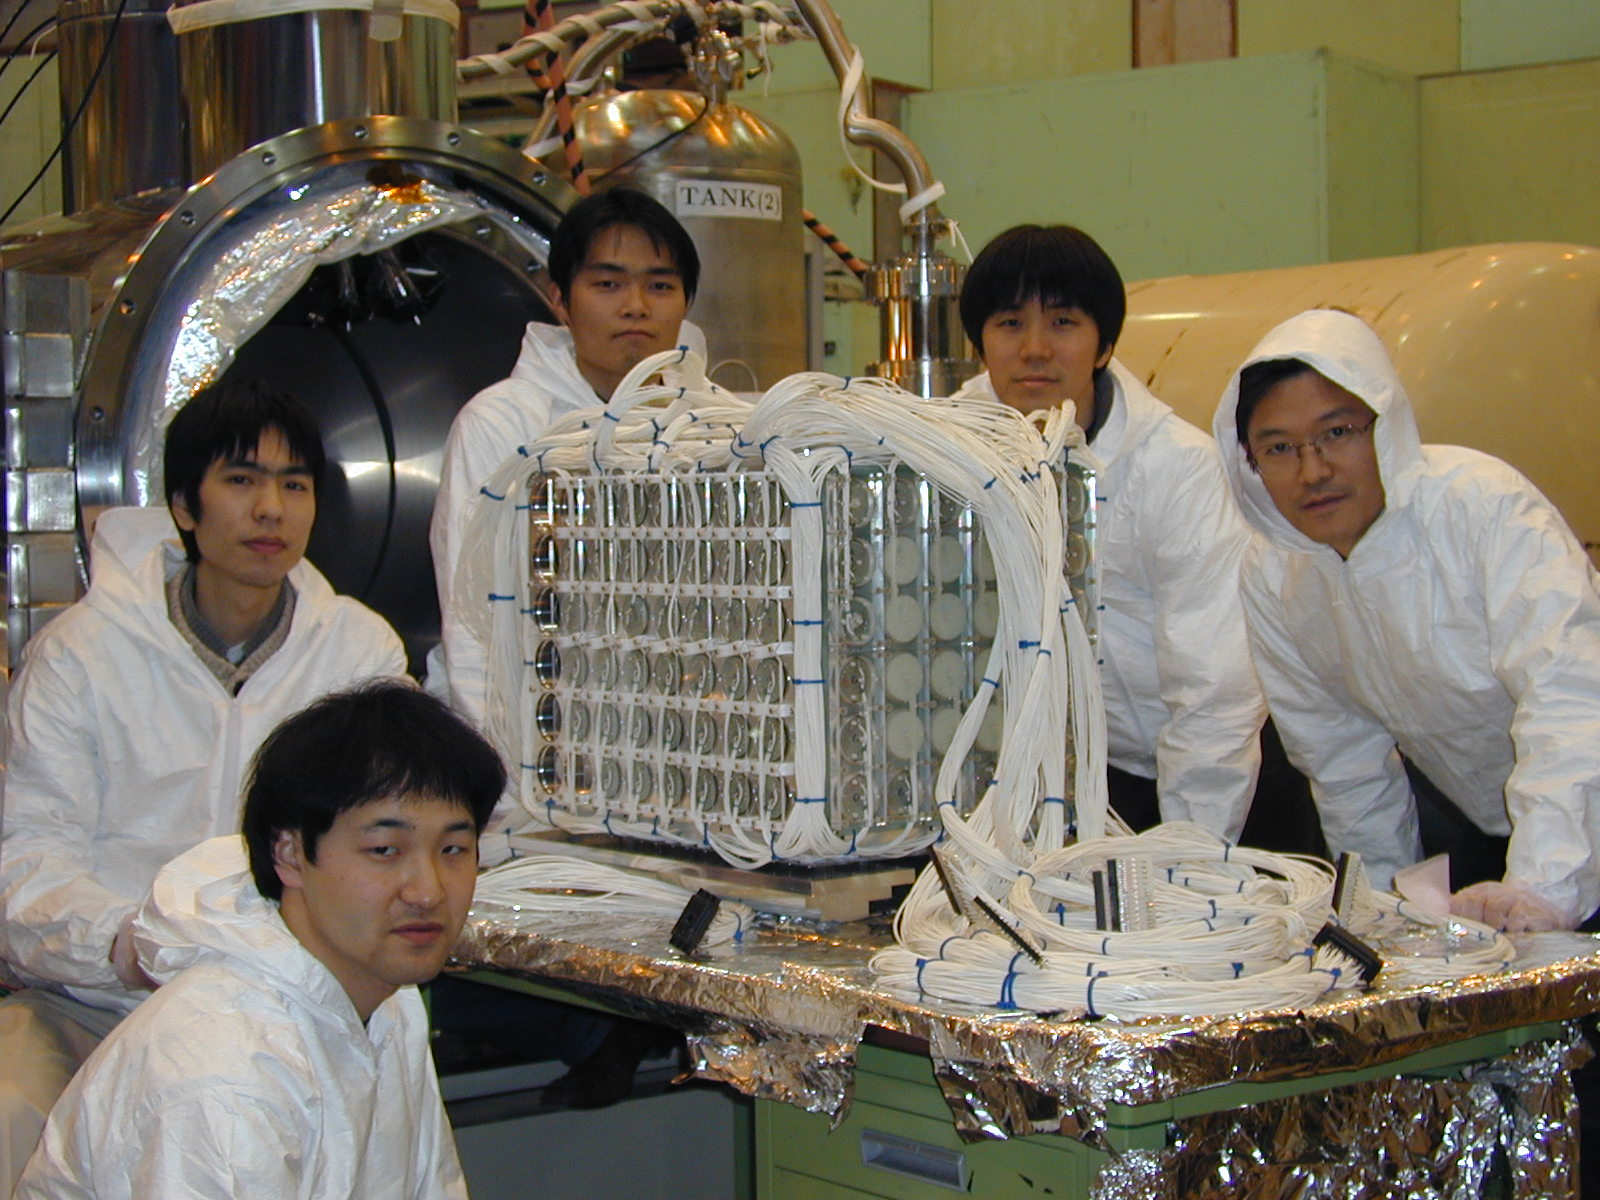
\includegraphics[width=0.9\columnwidth,clip]{fig/wataru.jpg}
  \caption{Large prototypeと呼ばれるMEG II液体キセノン検出器の試作器を試験する大谷さんたち。右から三原さん、大谷さん、西口さん、澤田さん、あと名前わからない人。三原さんと西口さんは現在KEKの研究者で、澤田さんは(ご存知の通り)ICEPPの研究者である。}
  \label{fig:wataru}
\end{figure}


%% \begin{figure}[h]
%%   \centering
%%   \begin{subfigure}[t]{0.45\columnwidth}
%%     \centering
%%     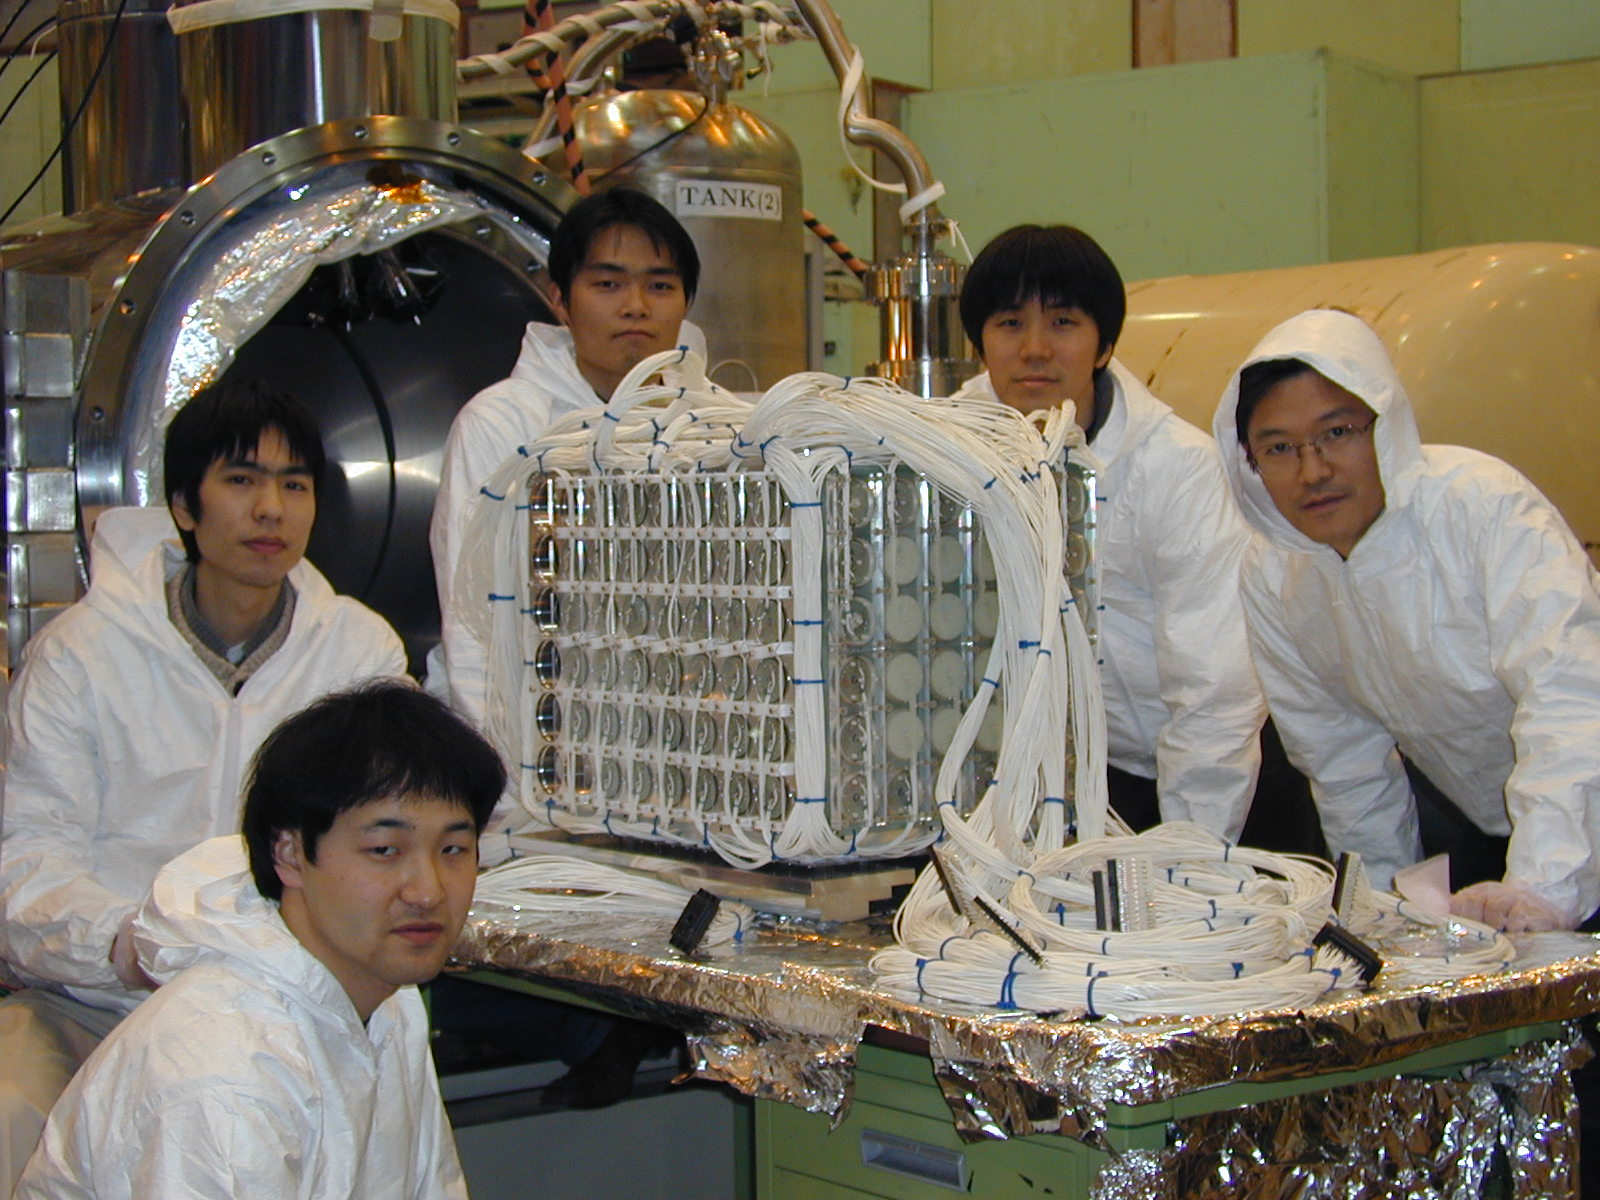
\includegraphics[width=\columnwidth,clip]{fig/wataru.jpg}
%%     \caption{}
%%     \label{fig:wataru}
%%   \end{subfigure}
%%   \hspace{0.1\columnwidth}
%%   \begin{subfigure}[t]{0.45\columnwidth}
%%     \centering
%%     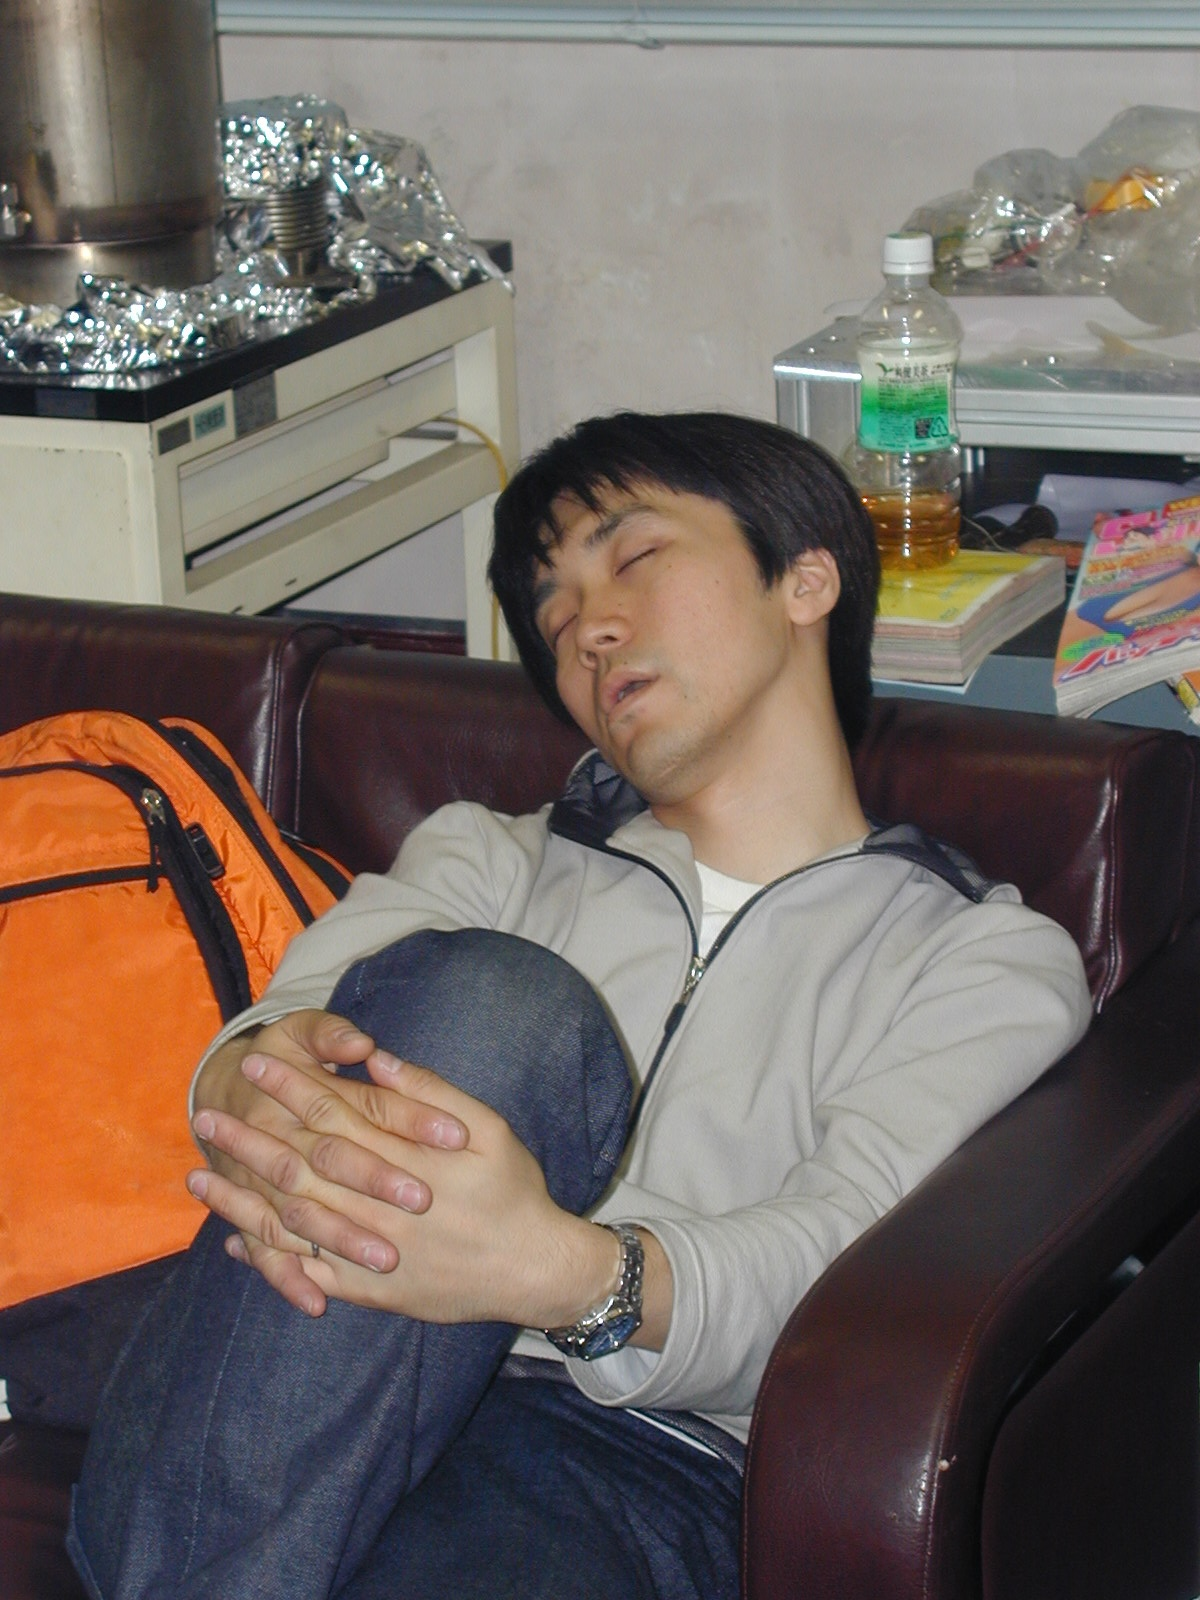
\includegraphics[width=\columnwidth,clip]{fig/wataru_sleeping.jpg}
%%     \caption{}
%%     \label{fig:wataru_sleeping}
%%   \end{subfigure}
%%   \caption{}
%%   \label{fig:wataru_summary}
%% \end{figure}


\begin{wrapfigure}{R}{0.3\columnwidth}
  \vspace*{-\intextsep}
  \centering
  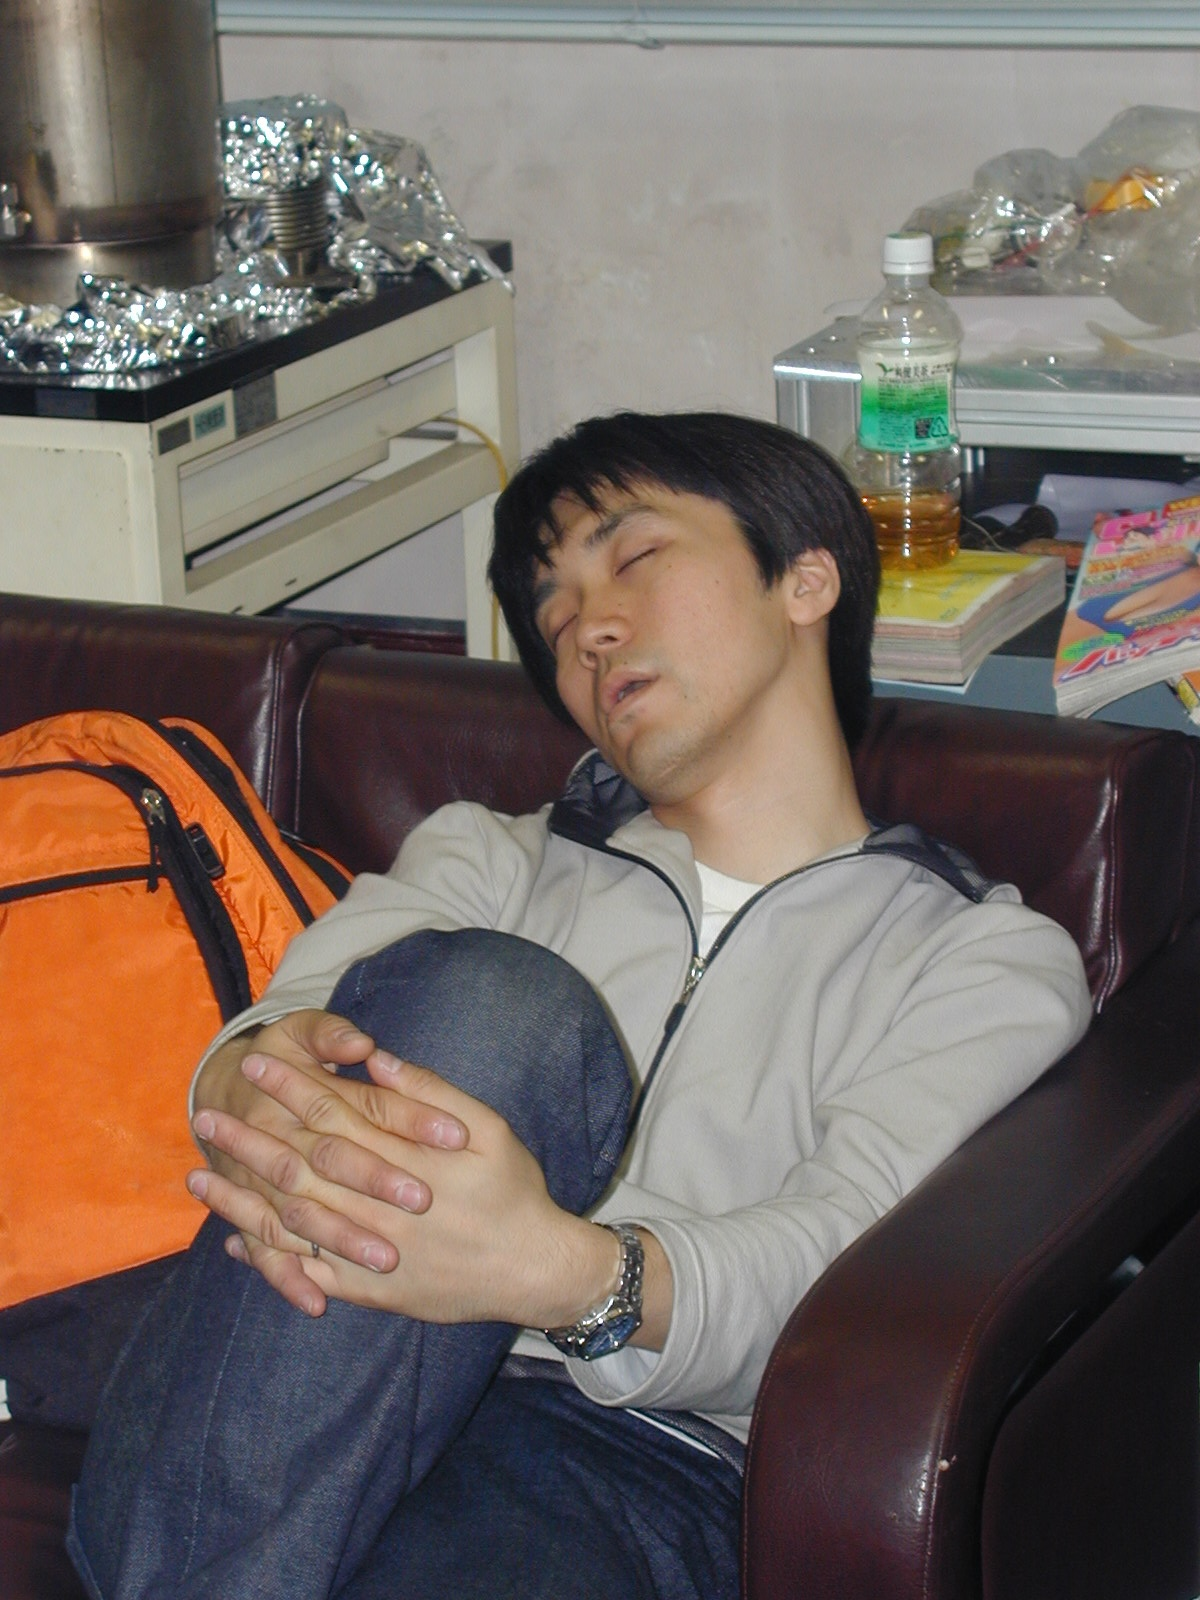
\includegraphics[width=0.3\columnwidth]{fig/wataru_sleeping.jpg}
  \caption{研究で疲れ果てて仮眠を取る若かりし頃の大谷さん。}
  \label{fig:wataru_sleeping}
\end{wrapfigure}


\subsection{岩本敏幸助教}
aaa
\subsection{Lukas Gerritzen特任助教}
aaa
\subsection{潘晟特任助教}
aaa
\subsection{大矢淳史特任助教}
aaa
\subsection{山本健介(D4)}
aaa
\subsection{村田樹(D4)}
aaa
\subsection{池田史(D3)}
aaa
\subsection{李維遠(D2)}
aaa
\subsection{小川拓泰(D1)}
aaa
\subsection{神山大樹(D1)}
aaa
\subsection{高津大誠(D1)}
aaa
\subsection{馬越隆成(D1)}
aaa
\subsection{榊原澪(M2)}
aaa
\subsection{清野拓己(M2)}
aaa



\renewcommand{\bibname}{引用文献}
\ifdefined\bynumber
\bibliographystyle{jecon6.5.1_by_number}
\else
\bibliographystyle{jecon6.5.1_by_name}
\fi
\bibliography{thesis}
\label{page:bib}


\end{document}

